\documentclass[10pt,draftclsnofoot,onecolumn]{IEEEtran}
\hyphenation{op-tical net-works semi-conduc-tor}

\usepackage[margin=.75in]{geometry}
\usepackage{courier}
\usepackage{ifthen}
\usepackage{setspace}
\usepackage{listings}
\usepackage[usenames, dvipsnames]{color}
\usepackage{tabularx}
\usepackage[strict]{chngpage}
\usepackage{cite}
\usepackage{graphicx}
\usepackage{acronym}
\usepackage{color}
\usepackage{makeidx}
\usepackage{url}
\usepackage{listings}
\usepackage{verbatim}

\makeindex

\acrodef{NPM}[NPM]{Node Package Manager}
\acrodef{OSU}[OSU]{Oregon State University}
\acrodef{AIAA}[AIAA]{American Institute of Aeronautics and Astronautics}
\acrodef{COCOM}[COCOM]{Coordinating Committee for Multilateral Export Controls}
\acrodef{AGL}[AGL]{Above Ground Level}

\lstset {
	language=C,
	basicstyle=\ttfamily,
	keywordstyle=\color{blue}\ttfamily,
	stringstyle=\color{red}\ttfamily,
	commentstyle=\color{OliveGreen}\ttfamily,
	morecomment=[l][\color{magenta}]{\#}
	showstringspaces=false,
	showspaces=false,
	frame=single,
	captionpos=b
}

\newcommand{\commandline}[2][\empty] {
	\begin{quote}
		\texttt{#2}
		\ifthenelse{\equal{#1}{\empty}}{}{\begin{quote}#1\end{quote}}
	\end{quote}
}

\newcommand{\sigline}[1][\empty] {
	\vspace{1in}
	\hrule width0.5\textwidth
	\vspace{1mm}
	\noindent #1
}

\newcommand*{\SignatureAndDate}[1]{
	\vspace{1in}
	\par\noindent\makebox[2.5in]{\hrulefill} \hspace{.5in} \makebox[2.0in]{\hrulefill}
	\par\noindent\makebox[2.5in][l]{#1}      \hspace{.5in} \makebox[2.0in][l]{Date}
}


\begin{document}
	\singlespace

	\title{\vspace{2in}Design}

	\author {
		Anisimova, Natasha
		\and
		Lee, Terrance
		\and
		Morgan, Albert
	}

	\markboth{CS Capstone 2016-2017}{Groundstation}

	\pagestyle{empty}
	\vspace*{2in}
	\begin{center}
		\huge
		Groundstation: Final Report\\
		\normalsize
		\vspace{5mm}
		\textbf{
			Team \#25\\
			High-Altitude Rocketry Challenge\\
		}
		\vspace{1mm}
		Natasha Anisimova\\
		Terrance Lee\\
		Albert Morgan
	\end{center}

	\vspace{5mm}

	\begin{center}
		\textbf{Abstract}
	\end{center}

	%\begin{adjustwidth}{0.75in}{0.75in}

	%Abstract goes here
	The \textit{Groundstation} software will collect telemetry from a rocket while it is in flight and graphically display the telemetry in real-time. Groundstation is made up several different components: collection of data, storage of data, interpolation of data, and
	display of data.
	This document is a compilation of most of the documents that were created over the course of the project.
	%\end{adjustwidth}

	\pagestyle{headings}

	\newpage

	% Uncomment this to make the table of contents
	\tableofcontents
	\newpage

\section{Purpose and Goals}
	In June 2017, the \ac{OSU} chapter of the
	\ac{AIAA} will launch a rocket at Spaceport America.
	This rocket will ascend to one hundred thousand feet \ac{AGL}.
	Designing, building, and launching the rocket will require the
	collaboration and expertise of dozens of engineers from a variety
	of disciplines, including mechanical, electrical, computer, and
	software.

	Many rockets record data during the flight. This data may include
	altitude, latitude, longitude, and more.
	Latitude and longitude
	data is helpful for locating the rocket after it lands, but
	if the data is located on the rocket, then it is useless
	for this task.
	Altitude data will tell the rocketry team if we have
	met the objective of one hundred thousand feet, but if the rocket
	is damaged or cannot be located for any reason, then the record
	of this achievement may be lost.

	However, the chicken-and-egg problem of not being able to access
	the location data before the rocket is found may be avoided by sending
	telemetry from the rocket in real-time.
	Telemetry may be received wirelessly
	by the rocketry team while the rocket is in flight, giving them
	access to useful information such as the rocket's last known location
	and the highest altitude reached. This telemetry will aid in the
	rocket's recovery and provide a log of the rocket's flight even if
	recovery is impossible.




	\section{The client}
	The project was requested by Dr. Nancy Squires, who is a senior
	instructor of mechanical engineering at Oregon State University.
	In addition to being a senior instructor, Dr. Squires runs many
	of the rocketry capstone projects.






% REQUIREMENTS





	\section{Introduction}

	\index{Purpose}
	\subsection{Purpose}
	This document will specify the requirements for the Groundstation (GS) software.
	It is intended for use by the OSU High-Altitude Rocketry Team.

	\index{Scope}
	\subsection{Scope}
	GS will gather telemetry from a rocket during flight.
	While the telemetry is being gathered, it will be logged and displayed graphically in real-time.
	This software will provide the following benefits to the users:
	\begin{enumerate}
		\item Real-time data will allow the rocket's location to be tracked during flight.
		Allowing this data to be accessed before recovery will aid in the recovery itself.
		\item The graphical display will make the data easy to interpret.
		\item Logging will allow the data to be analyzed at a later date.
		\item Altitude data will give evidence of whether the objective of one hundred thousand feet was met.
	\end{enumerate}

	\index{Definitions}
	\subsection{Definitions}

	\begin{itemize}
		\index{Accuracy}
		\item \textbf{Accuracy:} The absence of errors in the telemetry GS receives, logs, and displays.
		\index{Binary data}
		\item \textbf{Binary data:} Telemetry that represents one of two states, for example, ``stage 2 activated'' and
		``stage 2 not activated.''
		\index{Corruption}
		\item \textbf{Corruption:} The process by which data is altered or made unreadable.
		\index{Crash}
		\item \textbf{Crash:} A software crash; the event in which a piece of software ceases operation unexpectedly.
		\index{Die}
		\item \textbf{Die:} A process dies when it ceases operation and is removed by the operating system.
		The difference between dying and crashing is that a crash may cause the program to become non-responsive,
		whereas dying causes the process to end.
		\index{Groundstation}
		\index{GS}
		\item \textbf{GS:} Groundstation, the name of our software.
		\index{Graphical display}
		\item \textbf{Graphical display:} Data that is displayed using a visualization.
		\index{Live}
		\item \textbf{Live:} Updated in real-time.
		\index{Non-volatile storage}
		\index{Storage}
		\item \textbf{Non-volatile storage:} Storage that will not be erased when the system is powered down.
		For example, a hard drive or flash storage.
		\index{Page}
		\item \textbf{Page:} A web page that users of GS may connect to in order to view the telemetry.
		\index{Process}
		\item \textbf{Process:} A running program on a computer.
		%\index{Lean angle}
		%\item \textbf{Lean angle:} The angle relative to the vertical that the rocket is currently traveling.
		\index{Raspberry Pi}
		\item \textbf{Raspberry Pi:} A small, inexpensive computing platform.
		\index{Real-time}
		\item \textbf{Real-time:} Each telemetry datum received from the rocket must be processed and
		displayed in under one second.
		\index{Redundant sensors}
		\item \textbf{Redundant sensors:} Two or more sensors that provide the same type of data.
		\index{Reliability}
		\item \textbf{Reliability:} In the event of a software crash, the Groundstation software should automatically
		start and begin all normal functions in under five seconds.
		\index{Robustness}
		\item \textbf{Robustness:} In the event that GS receives data that is garbled or otherwise does adhere
		to the protocol, it must continue to receive and display data and not break the real-time requirement.
		\index{Storage}
		\item \textbf{Storage:} A device where data is logged.
		\index{Telemetry}
		\item \textbf{Telemetry:} Data received from the rocket while the rocket is in flight.
		\index{Telemetry packet}
		\index{Packet}
		\item \textbf{Telemetry packet:} The rocket will send a telemetry update once per second. Each one of these updates is a ``telemetry packet.''
		\index{Vizualation}
		\item \textbf{Visualization:} Information or data, transformed into an visual context.
	\end{itemize}

	\subsection{Overview}
	The rest of this document contains specific requirements about the functionality and constraints of GS. This includes
	the needs of the entire rocketry team, the physical constraints of the system, and the limitations of the launch site.

	\textit{Overall description} gives a high-level view of the functions of the software and describes any constraints.
	\textit{Specific requirements} gives a detailed list of requirements that were proposed by the OSU High-Altitude
	Rocketry Team and describes specific requirements and constraints.


	\section{Overall description}
	\index{Product perspective}
	\subsection{Product perspective}
	GS will receive data from a serial interface, via hardware and a protocol provided by the avionics team.
	Due to the launch site not having any connection to the Internet or mobile service, GS will not interact with
	any outside systems.
	Additionally, GS will provide a software interface that allows users to view the telemetry,
	graphically, in real-time.
	\subsection{Product functions}
	GS provides two major functions while the rocket is in flight:

	\begin{enumerate}
		\index{Logging}
		\item Telemetry logging to non-volatile storage.
		\item Display of real-time graphical data.
	\end{enumerate}

	\subsection{User characteristics}
	\index{Users}
	The users of this software will be limited to engineering students and advisors who are part of the OSU High-Altitude
	Rocketry Team.
	These users will be expected to be familiar with the software and the rocket launch.
	Because the software team works closely with the rest of the rocketry team on regular basis,
	any training necessary will be conducted in-person.

	\subsection{Constraints}
	\index{Constraints}
	\begin{itemize}
		\item Because of the remote nature of launch sites, the software must operate without an Internet connection.
		\item The software must be as reliable as is reasonably possible, and additional features must not compromise the reliability.
		\item Groundstation will receive telemetry via a protocol that is to-be-determined by the avionics team.
	\index{Browser}
	\index{Web browser}
	GS will support most modern desktop web browsers, including:
	\begin{itemize}
			\item Chrome version 54 or higher.
			\item Edge version 14 or higher.
			\item Firefox version 49 or higher.
			\item Safari version 10 and or higher.
		\end{itemize}

	\end{itemize}

	\index{Assumptions and dependencies}
	\subsection{Assumptions and dependencies}
	\index{Raspberry Pi}
	\index{Internet}
	\index{Raspberry Pi}
	Groundstation will run on a Raspberry Pi with no Internet connectivity.

	\subsection{Apportioning of requirements}

	\begin{figure}
		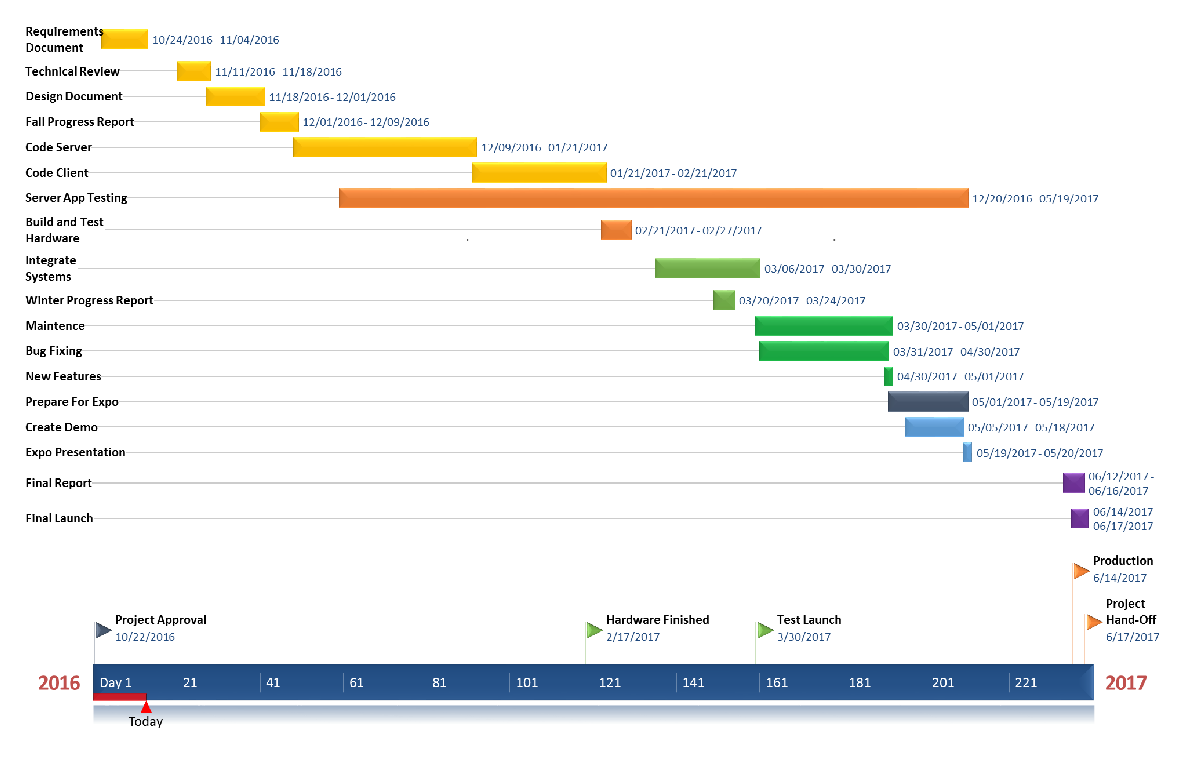
\includegraphics[width=\linewidth]{ganttchart.eps}
		\caption{A Gantt chart outlining the work to be done over the next nine months.}
		\label{fig:gantt}
	\end{figure}

	Figure \ref{fig:gantt} shows a gantt chart outlining our schedule from now until the first test rocket launch.
	Although the final rocket launch is on 23 June, all core systems of GS should be finished by the test launch in mid-May.

	\index{Specific requirements}
	\section{Specific requirements}

	\index{External interface requirements}
	\subsection{External interface requirements}
	\index{User interfaces}
	\subsubsection{User interfaces}
	Users will interact with GS by connecting via a web browser. The Raspberry Pi and other associated hardware,
	to be provided by the avionics team,
	will broadcast a wireless network that users will connect to and access GS through a web browser.
	From this page, users will be able to access the graphical display of the telemetry.

	\index{Hardware interfaces}
	\subsubsection{Hardware interfaces}
	GS will run on a Raspberry Pi broadcasting a wireless network. Users will connect to GS with their personal computers
	via the wireless network.

	Data is received from a serial interface using a protocol that will be determined by the avionics team.

	\index{System Features}
	\subsection{System Features}

	The stimulus for all specific requirements is receiving a telemetry packet. The specific responses to each telemetry packet are:
	\begin{itemize}
		\item GS will collect data from a serial interface using a yet-to-be-determined protocol designed by the High-Altitude Rocketry Team's avionics section.
		\item GS will log all telemetry in real-time to non-volatile storage so that it can be analyzed
		after the launch.
		The data from the serial port will be written to directly to non-volatile storage in order to limit
		the possibility of corruption.
		\item The graphical display shall be updated in real-time.
		\item Users will connect to GS and be able to view a visualzation of the telemetry in real-time.
		\item GS will support a live line graph visualization for altitude data.
		\item GS will have the ability to show the most recently recorded latitude and longitude in a numerical format.
	\end{itemize}

	\index{Performance requirements}
	\subsection{Performance requirements}

	\begin{itemize}
		\item When a new telemetry packet is received, GS will log the telemetry and update all visualizations in under one second.
		\item GS will support a minimum of 20 concurrent users.
	\end{itemize}



	\subsection{Design constraints}
	\index{Design contraints}
	\index{Contraints}
	\index{Raspberry Pi}
	GS will run on the hardware chosen by the avionics team at the beginning of the project.
	At a minimum, this hardware will be a Raspberry Pi 3 model B, which has a 1.2 GHz quad-core 64-bit ARM Cortex-A53 processor
	with 1 GB of SDRAM memory.

	\subsection{Software system attributes}

	\subsubsection{Reliability}
	\index{Reliability}
	In the event a GS process dies, a new process should begin and continue operation in under five seconds.

	\subsubsection{Robustness}
	\index{Robustness}
	If GS receives corrupted or otherwise incorrectly formatted telemetry, it should not crash.
	Additionally, the users should not be able to crash GS from the web interface.

	\subsubsection{Accuracy}
	\index{Accuracy}
	GS should not introduce any errors in the telemetry it recieves.
	Data should be logged and displayed with 100\% accuracy.

\printindex



%Blog post



\section{Development Log Fall 2016}

\subsection{Week 3}
\subsubsection{Anisimova, Natasha}
\begin{itemize}
	\item \textbf{Plans: For the following weeks we are hoping to communicate more with the Electircal Engineers so that
		we know what type of equipment we have to work with. Another bonus is that we will be getting recruits that could
		help us with creating the software.}
	\item \textbf{Progress: We created our first set of blog posts. Also, we created a problem statement that our team
		and our client agreed with. Meeting with the entire rocket team gave us a good idea how the work was going to split up
		between the individual teams. }
	\item \textbf{Problems: Knowing that we would not have Wi-Fi connection at the site, we would have to create our own
		solution as to how we were going to get the software to everyone on the team.}
\end{itemize}
\subsubsection{Morgan, Albert}
\begin{itemize}
	\item \textbf{Plans: }
	The plans for the coming week are to:
	\begin{itemize}
		\item discuss a proposed architecture and scope for our project
		\item collect user stories from the rest of the rocketry team
	\end{itemize}
	\item \textbf{Progress: }
	Progress is going well. Our client, Dr. Squires, was very pleased with our problem statement. Currently, we are working with the avionics team to hammer out the details of the project.
	\item \textbf{Problems: }
	Git is an amazing tool, but it does not excel in fast, remote, simultaneous collaboration. Compounding this with the large size of the rocketry team has made it difficult to produce the documentation in a timely manner.
\end{itemize}
\subsubsection{Lee, Terrance}
\begin{itemize}
	\item \textbf{Plans: }Next week we should meet a couple of more underclass men that couldn't make it to the meetings last week. Also we hope to get a little bit more precise information from each team. They should know more about the competition, materials, and so on that pertains to us. I personally will be joining the AIAA by the end of this week because they are one of our main sponsors plus they are helping me get my class one certification. Also meeting our TA for the first time next week.
	\item \textbf{Progress: }This week we were able to finish our problem statement. Do to my previous plans I had the job of redoing our abstract from when we had another group read our abstract and read it. I also did some proofreading and had the ability to allow someone who knows nothing about computer science or rocketry read it. They were able to understand what we were trying to get a crossed with our problem statement. We got a general idea of what each team from the project wants from us software wise. What the teams needs and their wants. That way we have primary and secondary objectives.
	\item \textbf{Problems: }I personally had some issues with some prior engagements. So I wasn't able to contribute as much until late Wednesday. That shouldn't happen again. My teammates were great to help with that. I had some issues with GitHub. I haven't had to use the command line ever. I am used to using source tree but I noticed I have more control with the command line. Keeping up with all the information of all the teams for the project is tough. They have information that can help us understand what is good for designing the software even if we aren't working directly with them. That's why it is good to know the verbiage of aerospace, rocketry, mechanical engineers and electrical engineers. I don't need to know everything but I should know at least what they are speaking so that I am not asking them to explain everything every time we have a conversation.
\end{itemize}
\subsection{Week 4}
\subsubsection{Anisimova, Natasha}
\begin{itemize}
	\item \textbf{Plans: }
	At the moment we have decided to create proof of concepts each week that we and the recruits will
	focus on in order to continue to progress further.
	\item \textbf{Progress: }
	We were able to recruit a few students to help us conduct research.
	\item \textbf{Problems: }
	So far we are unsure of how the Avionics team will be formatting the data and what protocol they
	will be using.
\end{itemize}
\subsubsection{Morgan, Albert}
\begin{itemize}
	\item \textbf{Plans: }
	The plans for the coming week are to:

	\begin{enumerate}
		\item	Figure out some of the details about our architecture, especially exactly how the application server should interact with the web server.
		\item Make a list of proof-of-concepts that need to be done
		\item Bring the rest of the students up to date on the overall architecture, and find some tasks for them.
		\item Write the requirements document.
	\end{enumerate}
	\item \textbf{Progress: }
	Progress is going well. We haven't started any development work yet, and there are still some critical pieces of the architecture that still need to be detailed, but we have a very good high-level view of what the architecture should look like. We have a number of other students who are involved in the rocket team that should be a terrific asset to our project.
	\item \textbf{Problems: }
	No particular problems this week, but after doing some research about application/web server integration, there appears to be a lot of different ways we could design our architecture, and I'm not sure how to decide which one is best for us.
\end{itemize}
\subsubsection{Lee, Terrance}
\begin{itemize}
	\item \textbf{Plans: }We were going to ask the team leads for some glossary terms and Dr. Squires for requirements. With the glossary terms we were going to take the ones that we felt pertained to our document and use them.
	\item \textbf{Progress: } We came to agreement that we needed to speak to get some terms from the whole team for the glossary because this wasn't just a CS project. Since this a project that takes collaborate of teams to succeed in this project we should need some of their terms too.
	\item \textbf{Problems: }After Speaking with Dr. Winters she said that our problem statement was at what she called level 2. That we needed to be just a little be higher on our overview to where we started. I had also ran into our TA and had him look at our problem statement for formatting errors since he has been an instructor to make sure we weren't doing anything wrong there. He said it was fine and gave me some feedback about the problem statement but it was the same as Dr. Winters.
\end{itemize}
\subsection{Week 5}
\subsubsection{Anisimova, Natasha}
\begin{itemize}
	\item \textbf{Plans: }
	We will have to finish the requirements document and have a separate meeting for the recruits.
	\item \textbf{Progress: }
	We created a draft for the requirements document.
	\item \textbf{Problems: }
	Researching how to create a Gantt chart for free took a lot more time than expected. We also were
	having a problem with boring our recruits with senior design work, so we created a separate time to meet with them.
\end{itemize}
\subsubsection{Morgan, Albert}
\begin{itemize}
	\item \textbf{Plans: }
	The plans for the coming week are to:
	\begin{itemize}
		\item finish the requirements document
		\item develop a better workflow process to prevent near-disasters during busy weeks
	\end{itemize}
	\item \textbf{Progress: }
	This week, we wrote the draft for the requirements document. Given the open-ended nature of our project, it was difficult to decide what should go in this document and what should go in a design document. We ended up leaving many implementation details, which are already planned but not part of the actual requirements of the project, for the design document.
	\item \textbf{Problems: }
	It was a crazy week with the career fairs, and we almost didn't get everything done that we needed to. We managed to pull through, though.
\end{itemize}
\subsubsection{Lee, Terrance}
\begin{itemize}
	\item \textbf{Plans: }
	Next week do a little more research for the final product of the requirements document. This way it will be clean and concise. When that is finished start thinking about the next document if we have time.
	\item \textbf{Progress: }
	We were able to get some feedback from the other sub-teams about what they require from us on the software side. Did some research about about what is needed from real software engineers just to get a little more familiar on how it works when dealing with multiple teams. I found out the biggest issue is communication and everyone wants their section to come first at the beginning. What successful teams do is come to a realization on one overall plan and do what is best for the overall team not for themselves.
	\item \textbf{Problems: }
	The requirements document was more difficult then I thought it would be. Since we are getting request from other sections of the team. We have to decipher what should and what should not go into this. Also it makes you actually think about what needs to go into something that needs to work not just for you or your team but for a whole project on a big scale. Since this is something that no other collegiate team has done we don't have much to go with so we are thinking about this should work at this moment but we may research something later and it may not work later. It kind of sticks a little bit in the back of your mind is this a waste of time or is this the right thing that we are doing. The nice thing about research type things like this you will never know until you try.
\end{itemize}
\subsection{Week 6}
\subsubsection{Anisimova, Natasha}
\begin{itemize}
	\item \textbf{Plans: }
	GS is the name of our software. I am planning on creating some kind of logo for it that way we can put it up into our web application.
	\item \textbf{Progress: }
	We finished the requirements document. I also spoke with a Computer Visualization person, Nik, that Winters introduced me to. He mentioned that we could get the topology and satellite images of the area from Professor Mike Bailey. The texture image can be mapped to the topology and we can use that for our web application. He also mentioned that it would be cool if we could get an PC to actually have the web server on. Kirsten added that there could be possible funding for this as well. We also realized that we pretty much have four months before the test launch. A lot needs to happen before now and then.
	\item \textbf{Problems: }
	We do not have a lot of time left before the test launch.
\end{itemize}
\subsubsection{Morgan, Albert}
\begin{itemize}
	\item \textbf{Plans: }
	We've been so busy with the requirements document the last couple weeks, I have no idea what we are going to bring to the meeting on Monday. The current plan is to make a plan.
	\item \textbf{Progress: }
	This week, we finished the requirements document. Because of the amount of work the requirements document needed, we did not progress in any of our other areas.
	\item \textbf{Problems: }
	The requirements document needed extensive revisions, and I think we could have used another week to make it even better. We don't have a customer who dictates exactly what they want, so we had to make a lot of decisions about where to take the software before we could write the requirements for it.
\end{itemize}
\subsubsection{Lee, Terrance}
\begin{itemize}
	\item \textbf{Plans: }Next week we are going to do more research on the software as well as the parts that we are in particular charge of for the technical document.
	\item \textbf{Progress: }We finished our requirements document this week. I originally had to take care of the availability, reliability, and Design constraints. We came to an understanding that we didn’t need availability and to shorten the reliability to what it’s base of what needs to really do. Natasha came up with a beautiful Gantt chart. We also came up with a name for our software too which we are all really happy about. We used the extra day to proofread our document to make sure we had it in order too.
	\item \textbf{Problems: }I think the biggest issue with the requirement document was trying to choose what was needed and what wasn’t need for our project. Our project is a little different because we get requirements that there one week but then the next week we find out that is not going to work and we have to change it. So we had to generalize what is going to needed.
\end{itemize}
\subsection{Week 7}
\subsubsection{Anisimova, Natasha}
\begin{itemize}
	\item \textbf{Plans: }
	Up until Monday we will be finishing the technical document and after that we will be moving on to the design document. So far we have a lot of ideas from the team with the user stories. There will be several stretch goals we can pull from them but some that we can actually implement.
	\item \textbf{Progress: }
	When speaking to Professor Bailey about visualization, on behalf of the technical document, he mentioned that a GoPro Dual Hero System could be placed on the rocket as an interesting addition. This 3D capturing camera would give a new and innovative way of looking at space. It would also be the first time that it has been used on a rocket, but it has been used in skydiving in the past.
	\item \textbf{Problems: }
	We have also found out that getting to 100k ft will not be a challenge anymore from the ME teams. Our problem now is staying under 135k ft. It sounds like that will not be too much of a problem considering the fact that weight can always be added to slow down the rocket. Due to the overshot we also have to account for that when considering the type of data, we will still be receiving at that height. Thankfully we can still come up with an estimated altitude, velocity, and location from the other sensors.
\end{itemize}
\subsubsection{Morgan, Albert}
\begin{itemize}
	\item \textbf{Plans: }
	This week we will work on the technical review and start making some decisions about the components we will use in our software. We also need to start making some decisions soon so we can keep the interest of the rest of the people in our team.
	\item \textbf{Progress: }
	This last week we finished the requirements document. It was difficult to nail down specific requirements for this project. Our job is to work with the rest of the rocketry team to make a piece of software that we are all happy with, and didn't start out with a lot of hard requirements from the client.

	One of the non-capstone members of our team has decided to work on a predictive positioning system that will show an estimate of where the rocket is in the case that we lose GPS data. The event of a data loss is likely due to restrictions put on GPS devices to prevent people from building missile guidance systems. During certain portions of the rocket's flight, we will be going too fast or too high for a civilian GPS to work due to these restrictions.
	\item \textbf{Problems: }
	There were no problems this week. The technical review is a straightforward document and I do not anticipate any problems.
\end{itemize}
\subsubsection{Lee, Terrance}
\begin{itemize}
	\item \textbf{Plans: }
	I want to finish the technical document this weekend so that we can look forward to the design document phase. I believe that will be really interesting with this team I really cannot wait to see what we come up with.
	\item \textbf{Progress: }
	This week we our TA told us we did well on the requirements document. This lead us to be able to split the technical document up easily. We decide first to split the document up in a way that were each one of us chose things that we would enjoy. That way it would be easier on each other to do our part of this document. For my part I have been doing research to make sure that they are the best for each section. Also since we are working with other disciplines I have spoken to the others that are involved in with each of my part to make sure that this is what we are doing and these are the sensors that they are using.
	\item \textbf{Problems: }
	The main problem that I have ran into is the research on retrieval. The reason I say that is because I am looking at the different languages and there are so many different ways that people code. I am just trying to find which one would be the best in this case.
\end{itemize}
\subsection{Week 8}
\subsubsection{Anisimova, Natasha}
\begin{itemize}
	\item \textbf{Plans: }
	This Monday we are going to have to make sure we agree with everything that is in the technical document so what we can actually start programming. Also a lot of work needs to go into how we will be able to calculate the rocket's location based off the other sensors on the rocket. The GPS signal will be cutting out during the initial launch and after it reaches a certain height. I want to simple create demo with WebGL and put it up. This would be a good little test to see if everyone on the team has browsers that support WebGL. We also have a chance to get our capstone group interviewed and filmed by Rachel. Kirsten Winters sent me an email about the opportunity and now we are waiting on the okay from Dr. Squires.
	\item \textbf{Progress: }
	Technical document got submitted on time. We did get an extension from Kirsten but thankfully we didn't end up needing it.
	\item \textbf{Problems: }
	We did have a problem with working on the technical document and making sure that it flowed. Also if we start earlier on it, it would help with making sure that we are all on the same page. I definitely need to work on putting up a draft of my work early on so that the rest of the group knows what I am thinking.
\end{itemize}
\subsubsection{Morgan, Albert}
\begin{itemize}
	\item \textbf{Plans: }
	This week we need to begin work on the design document. The design document is very precise and complete, and I anticipate that this document will be a lot of work, so we should get started early. Additionally, we finally need to make some decisions about the technologies we are going to use, so we need to have a discussion as a group to finalize these decisions.

	Additionally, we need to figure out a better workflow so we don't have any last-minute problems (see "problems", below).
	\item \textbf{Progress: }
	This week we finished the technology review. It barely got done in time, and Natasha and I spent a lot of time fixing it for the final submission.
	\item \textbf{Problems: }
	We had problems with this week with last-minute work that didn't follow the existing template, and also from lack of communication. We need to set up a more rigorous method for quality assurance with our documents. I believe that I need to personally start the documents early and set up the sections for people to fill in to prevent situations where I have to manually edit other people's work to conform to standards in the future.
\end{itemize}
\subsubsection{Lee, Terrance}
\begin{itemize}
	\item \textbf{Plans: }Next week to catch up with my team from everything I missed with being out of town. Also I am going to recommend that we have more than one meeting a week while working on this design document since our meeting is so early during the week.
	\item \textbf{Progress: }We finished the technical document this week. We are now onto the design document. Since I missed class on Tuesday from being out of town and missing our meeting with our TA I made an extra appointment with him. I went over a what I missed and how should the design document be approached. I wanted to make sure that this is done well so that we go into the programming part of this with a good design and we have less debugging.
	\item \textbf{Problems: }I had an issue with having a interview in another state but I feel that with these more precise documents that one meeting a week isn't enough. We had some issues with the technical document that due to being out of town that I haven't been able to speak to my team about but I feel if we have more meetings to go over the design document as we work on it we can fix those issues.
\end{itemize}
\subsection{Week 9}
\subsubsection{Anisimova, Natasha}
\begin{itemize}
	\item \textbf{Plans: }
	This last Monday we went over what should be in the design document, making sure to cover what we had already written.
	\item \textbf{Progress: }
	\begin{table}[htbp!]
		\centering
		\caption{My caption}
		\label{my-label}
		\begin{tabular}{lll}
			\hline
			\multicolumn{1}{|l|}{Tech Review} & \multicolumn{1}{l|}{Requirements Review} & \multicolumn{1}{l|}{Viewpoints}  \\ \hline
			\multicolumn{1}{|l|}{Web Server}  & \multicolumn{1}{l|}{Raspberry Pi}        & \multicolumn{1}{l|}{Interaction} \\ \hline
			Web Backend                       & Real-Time                                & Resource Management              \\
			Logging                           & Reliability                              & Interface                        \\
			Data Visualization                & Corruption                               &                                  \\
			UI Interaction Model              & Accuracy                                 &                                  \\
			UI Interface Organization         & Redundant Sensors                        &                                  \\
			Retrieval                         & Storage                                  &                                  \\
			UI Toolkit                        & Internet/HAM                             &
		\end{tabular}
	\end{table}

	\item \textbf{Problems: }
	Splitting up the work seems like the most difficult thing. Also it being Thanksgiving break it is hard to know when everyone is free or available to work on the assignment.
\end{itemize}
\subsubsection{Morgan, Albert}
\begin{itemize}
	\item \textbf{Plans: }
	This week we are going to hammer out the design document, as well as any other things we need to do. We have a pretty good idea of what the design is going to be, but we may change our mind as we start writing it, so it's important here to be flexible.
	\item \textbf{Progress: }
	This week we actually starting working on the design of our software. On Monday we went over, in detail, how we are going to write the design document, and which viewpoints we should use.
	\item \textbf{Problems: }
	Due to the nature of the design document assignment description, I'm still not sure exactly how we are going to divide the work up. It would be fairly trivial to just divide the work evenly, but because we all have to do the sections that we did in the technology review, some elements, such as relationships between two different technologies that were described by two different group members.
\end{itemize}
\subsubsection{Lee, Terrance}
\begin{itemize}
	\item \textbf{Plans: }As I have started early on the design document and have read the template a little more in detail. It seems that some of the design viewpoints are not fit for certain components and we should talk about this on our Meeting with our TA on Monday as well as our team meeting.
	\item \textbf{Progress: }This week we broke down the design document before the Thanksgiving Break. That way we knew which areas of the document we were going to use and could get an early start on it. We did notice that not all components have the same areas. I have started some research and a rough draft on this document. We ran into an issue on the last one and I do not want us to run into the same thing again so I started early.
	\item \textbf{Problems: }As I read over our technical document and have read over the IEEE design document I have noticed that some of us are going to be writing more than others. I know that this is supposed to be split up into an individual sections but it does not seem fair that way. I do not think that if I finish early that I should not be able to help my other team members finish there component if they need it. I feel that this is what teams are here for.
\end{itemize}
\subsection{Week 10}
\subsubsection{Anisimova, Natasha}
\begin{itemize}
	\item \textbf{Plans: }
	Now that we have the Design Document out of the way, we can focus on the progress report. I got a very simple outline of what it will look like in PowerPoint but we still have a lot of work to do. The weekend will be dedicated to finishing that up as well as studying for final exams. Over the break I want to spend a lot of time creating the 3D environment that will be hosted on our website for the launch/tracking of the rocket.
	\item \textbf{Progress: }
	We had Dr. Squires sign the Design Document which was thankfully finished on time. Also, I think everyone is on the same page about using JavaScript for our software (node.js, three.js, etc.).
	\item \textbf{Problems: }
	Finishing the Design was a bit stressful. I had a couple errors with making sure the figures showed up on the right page. Spacing of pages was a big issue. I got a detailed email from Jon, the TA, about how all of that worked so my hope is that it will not ever happen in the future. Now that this term is almost over and future terms will not be as heavily loaded, I want to be able to finish things earlier than we have been in the past.
\end{itemize}
\subsubsection{Morgan, Albert}
\begin{itemize}
	\item \textbf{Plans: }
	The weekly rocket meeting has been canceled, so there is no coordination with the larger group that needs to be done. However, we plan to get at least some work done over the break. We should be able to get at least a basic running version of our software up in that time.

	Over the weekend we should be able to finish the content of our video and record it on Monday. We plan to break the presentation into bite-sized pieces for ease of recording and editing. Additionally, this will allow us to reuse some of the pieces for later presentations.
	\item \textbf{Progress: }
	This week we finished the design document. We've created the framework of our presentation, but we haven't started recording anything yet. The bones of our presentation has been created, but much of the content remains to be filled in.
	\item \textbf{Problems: }
	We only finished the design document at the last minute, which lead to some difficulties. If you ever find yourself in a situation where you are making GitHub commits before you have had your coffee, something has gone terribly, terribly, wrong. In order to prevent this in the future, I believe our team should institute a rigid internal timeline that ensures that work isn't being done hours before our deadlines. Over the break, I will look more into GitHub issues to see if they would be a useful tool for this kind of thing.
\end{itemize}
\subsubsection{Lee, Terrance}
\begin{itemize}
	\item \textbf{Plans: }Monday we plan to meet up to get the video done for the progress report.
	We plan on doing some coding over the break. My personal goal over the break is to learn node because I have never used it before and since that is our language for everything I figure it would be good to know how to use it.
	\item \textbf{Progress: }We got the design document done. Also Al made the base for the progress report.
	\item \textbf{Problems: }The design document took longer to finish than expected. Even though we had two weeks to do it. After reading it over the holiday many times it was still confusing and it seemed that we had many questions that never got quite answered. To prevent this we should probably meet up and have a group work session on documents, code, or whatever at least once a week where we are just working on the what needs to be done together in the same room. That way if things change or if we have questions we can solve them with each other. Also we are knocking a big chunk out right there with each other.
\end{itemize}

\section{Development Log: Winter 2017}
\subsection{Week 1}
\subsubsection{Anisimova, Natasha}
\begin{itemize}
	\item \textbf{Plans: }
	We hope to meet up with the rest of the team soon just to find out where everyone is since we last met and make sure that we are all on track. Also, I plan on working on the code and getting the images for the buttons we will have for the buttons and dials we will be using.
	\item \textbf{Progress: }
	Al wrote some code over break. I researched a bit more about the details of the user interface that we are trying to create. Unfortunately, I did not get as much as I wanted to over break.

	\item \textbf{Problems: }
	Snow days have set us behind in meeting with the entire team but we will have a chance to meet up with them this next Tuesday.
\end{itemize}
\subsubsection{Morgan, Albert}
\begin{itemize}
	\item \textbf{Plans: }
	The plan for this week is to get everybody on track for winter term. Last quarter, we had a lot of written assignments to complete, so it was easy to know what we were supposed to be doing at any given time. This quarter, we will need to be much more proactive and self-directed, so we will need to come up with a solid plan for how we will finish our project.
	\item \textbf{Progress: }
	Over the break I looked into task tracking and wrote a little bit of code for the groundstation backend. The most important feature for a task tracking system is ease of use. Much like source control, the best task tracker is the one that you use. An overly complicated or inconvenient task tracker won't do anyone any good, because no one (including me) will check their tasks. I looked into waffle.io, but it didn't seem to add any features that GitHub Projects didn't have or could easily replicate. Because we use already GitHub for everything else in our project, including source code, documentation, and blogging, GitHub Projects is the best option.

	I also started writing some of the backend over the break. It would make sense to use the node package manager (npm) to track client-side JavaScript libraries as well as server side, but making them accessible from the default /node\_modules path is tricky. I wrote some code that takes a list of JavaScript libraries, automatically finds them in the /node\_modules directory, and makes them available on the /scripts route.
	\item \textbf{Problems: }
	We usually do our meetings on Mondays, so the snow day on the first day of class and now MLK Jr. Day have set us behind. Hopefully we can meet on the Tuesday after MLK Jr. Day and start some real progress.
\end{itemize}
\subsubsection{Lee, Terrance}
\begin{itemize}
	\item \textbf{Plans: }
	Monday Al and I plan on meeting during MLK day to start going over the server and hopefully start some coding. I believe we will also have our meeting with the rest of the High Altitude Rocket team as well.
	\item \textbf{Progress: }
	Over the break I started to learn more about Node JS because we came to a consensus that it would be easier to use one language instead of multiple for the server. I have never used it so I figured it would be good to do research and learn as much as I can so I wouldn't be behind when we got into the guts of coding during this term.
	\item \textbf{Problems: }
	Due to the Snow and the MLK day trying to get our Rocket team meetings has been tough. Monday the normal days for all our meetings. We have been trying to be adjustable so that we can get on schedule and get this thing going.
\end{itemize}

\subsection{Week 2}
\subsubsection{Anisimova, Natasha}
\begin{itemize}
	\item \textbf{Plans: }
	Currently working on getting a complete 3D model of the rocket from the rest of the team. Some parts are still being changed. Continue working on scaling the 3D environment for the web user interface.
	\item \textbf{Progress: }
	We were finally able to meet with the rest of the team this Tuesday and schedule a regular meeting time with the TA. We also now have a solid launch rail group that will be working with us for the rest of the project.
	\item \textbf{Problems: }
	I had a family emergency come up this week. It involved me being away from the university for a few days.
\end{itemize}
\subsubsection{Morgan, Albert}
\begin{itemize}
	\item \textbf{Plans: }
	The one critical part of the software that is still missing is the encoding of the telemetry packet received via USB. We need to communicate with the ECE team to figure out what that is going to be. Additionally, we should be getting some hardware this week that will allow us to run our software on its target platform.
	\item \textbf{Progress: }
	This week I finished the "event chain" part of the backend. A new client connects via websockets, which fires an event. That event attaches a new event handler to the telemetry packet receiver, which causes the receiver to send the data to that client every time a packet is received. That, in turn fires a new event on the client side, allowing the backend to communicate with the frontend.
	\item \textbf{Problems: }
	No problems with the software this week. Despite class being canceled on Monday, we managed to have our weekly meeting with everyone there on Tuesday. Scheduling my upcoming wedding around the launch might involve some low-margin-of-error travel plans, but I believe it will work out.
\end{itemize}
\subsubsection{Lee, Terrance}
\begin{itemize}
	\item \textbf{Plans: }
	We have a laptop computer that we are getting on Tuesday to use for testing. After speaking with Al he suggested to ask Mr. McGrath for another Raspberry PI because he had a great Idea for testing it and the computer in one place. A type of Endurance testing to make sure if works the program will work for hours.
	\item \textbf{Progress: }
	We met with the rest of the team to get updated and we had our updated meeting with John Dodge our TA. We were able to get some feedback about our video and last report. I was able to speak to both Instructors about how we are doing in our project. I was able to get us a Raspberry PI so that we can test on from Mr. McGrath.
	\item \textbf{Problems: }
	The main problem this week was the holiday. Almost all of our meetings are on Monday and changing schedules to make meetings to fit around each others schedule so that we could meet with each other and the TA as well with the High Altitude group was very difficult.
\end{itemize}

\subsection{Week 3}
\subsubsection{Anisimova, Natasha}
\begin{itemize}
	\item \textbf{Plans: }
	I have a gyroscope and Arduino 101 that we can use for testing. For this upcoming week I plan on getting the height map to display in a web browser and possibly integrate it with what Terrance and Albert have done so far with the interface. Satellite images have proven to be more difficult to find. Professor Bailey agreed to help me since all I have found so far are lithography maps of the area with strange legends. We also have an undergraduate that is doing research on predicting where the rocket will land based off the initial data that we get from the sensors before takeoff.
	\item \textbf{Progress: }
	In the next couple days I'll have the height map of the area that we will be launching from and I'll be able to put it into the code that we currently have. This will give us a better display. We got the communication protocol from the ECE team today as well.
	\item \textbf{Problems: }
	I do not have the right satellite images for the area but I will be working with Professor Bailey to find them. It also looks like I will be the only one from the CS capstone team that will be able to go and stay for our launch.
\end{itemize}
\subsubsection{Morgan, Albert}
\begin{itemize}
	\item \textbf{Plans: }
	This week we got the Raspberry Pi, so we can begin to figure out how we are going to configure the operating system on the final project. Additionally, we should be getting a solid specification for the telemetry protocol from the ECE team this week, so we can begin to build the part of the application that receives that data.
	\item \textbf{Progress: }
	This week I worked out a bug in the JavaScript. The client was connecting properly when it was my computer connecting, but not when any other computer would connect. I checked my firewall settings, tried running the server in multiple operating systems, and it still didn't work. It turns out that I had hardcoded the "ws://localhost" address directly into the client when it makes the websocket connection.
	\item \textbf{Problems: }
	It looks like I may not be able to make the launch. I was told my several different people in the team's leadership that the launch would be on June 23, and I planned my wedding around that date. However, it turns out the launch will be on the 24th, and unless I reschedule my wedding I wouldn't be able to make it back to Oregon in time. This won't affect the timeline of the software, but it is a minor hiccup.
\end{itemize}
\subsubsection{Lee, Terrance}
\begin{itemize}
	\item \textbf{Plans: }
	Since we have a Laptop and a second Raspberry PI we are can test parts of the software as we build it to see how robust it really is. Code then test. Code then test. That way we if find a bug we can find it early then later in the program.
	\item \textbf{Progress: }
	This week we got some actually code working where the client can connect to the server. AL did that part. I was able to get us a Laptop for testing as well as another Raspberry PI. Also I have contacted the Avionics ECE team. They are supposed to be emailing me the protocol for all the components of what the rocket sensors are going to be sending back and the times.
	\item \textbf{Problems: }
	I am having an issue with getting the protocol from the ECE team. They said they were going to give it to me on Thursday but they did not send it to me. Luckly I know most of them from being an ECE previously so I was able to ask for it. Hopefully if I do not get it tonight I can get it this weekend.
\end{itemize}

\subsection{Week 4}
\subsubsection{Anisimova, Natasha}
\begin{itemize}
	\item \textbf{Plans: }
	We will be needing to create the OneNote document this upcoming week and register for the engineering expo. Any revisions that need to be done will be discussed during our Monday meetings. During that time, I am also hoping we will be able to select a team captain. We are planning on getting an SD card as well.
	\item \textbf{Progress: }
	I made a demo of the bump-mapping and displacement mapping in order to get a good understanding of what was happening in the code. I also have started to code with WebGL and will be slowly integrating it with what the rest of the group has up on Github. We are now all able to edit and add on to the code since Al made a small tutorial on how to allow extremely long file path names.
	\item \textbf{Problems: }
	There are a couple problems with trying to test the Web Server at the university over its network. Al talked to Kevin about it and unfortunately it looks like we will be needing to go through the IT department and wait for them to approve us (let us past OSU's firewalls). Since Kevin is on the committee we hope that we have pretty high chances of them granting the permissions for our team.
\end{itemize}
\subsubsection{Morgan, Albert}
\begin{itemize}
	\item \textbf{Plans: }
	We got the protocol from the ECE team late last week, so we plan on implementing that soon. Additionally, we finally got a bunch of class related non-code work, such as selecting a team captain, creating a One Note document, and sending team information to the expo organizers.
	\item \textbf{Progress: }
	This week we made some changes to the JSON format and how the data will be logged. Originally, we intended to log using a JSON format, because we were converting the data to JSON anyway, and storing it as JSON will make it easy to load. However, storing the data as JSON creates problems with terminating characters not being present if the program shuts down mid-operations. Storing the data as comma-separated values instead will maintain the integrity of the log even in the event of an unscheduled shutdown and make it easy for people to load into programs such as Microsoft Excel.
	\item \textbf{Problems: }
	We had a problem testing the web server on the university Wi-Fi because internal connections are blocked. I believe the simplest way to get around this is to broadcast our own Wi-Fi network to test on. This will be a better solution, anyway, because the final product is designed to run on an isolated Wi-Fi network. This does mean, however, that I will have to haul around more equipment on Mondays, when our team meets.
\end{itemize}
\subsubsection{Lee, Terrance}
\begin{itemize}
	\item \textbf{Plans: }
	We got work from the instructors on putting our "paperwork" in one note file. We have not voted on a team captain but I hope by Monday of next week we should have that done. With the Logging we are transferring it to a CSV file. It seem that the rest of team really liked that Idea. Also Natasha said she can work with that as well. I should have that done by Sunday at the latest unless some serious problem shows up.
	\item \textbf{Progress: }
	This week I am doing some additions to the Logging of the server. Al also found out why we could not log onto the server at OSU. It has something to do with the college's firewall. It works fine from his house so we should not have an issue when we are at the launch site.
	\item \textbf{Problems: }
	I believe that their was a problem with One Note. We got an Email from Dr. Winters about holding off on sending her our link. Also Al had an issue with the Rasberry PI not having a micro SD card. He asked Mr. McGrath for one. If he does not have one we are just going to have to pick one up ourselves.
\end{itemize}

\subsection{Week 5}
\subsubsection{Anisimova, Natasha}
\begin{itemize}
	\item \textbf{Plans: }
	Every Monday we are going to be putting everything that each of the separate branches has, take care of any conflicts, and merge everything into the master branch. This way both sides have an updated version of the project. We will have to revise some documents since several of our design decisions have changed since we wrote the document back in Fall term. I will be added more code over the weekend, unfortunately this week was a bit hectic with exams.
	\item \textbf{Progress: }
	The code for the WebGL Canvas now co-exists with the rest of the server. Due to the fact that everything needs to be integrated, we have split the project into two branches. There is a separate demo where the width of the WebGL Canvas changes depending on the user's browser size. This will insure that the user will not be missing anything. Vertex and fragment code for displacement mapping can be divided up into separate files so the code is more manageable.
	\item \textbf{Problems: }
	One problem that I have run into is making sure that my code does not have any web dependencies. In the end it seems like most things we can just download but then that means just filling up more memory on the Raspberry Pi.
\end{itemize}
\subsubsection{Morgan, Albert}
\begin{itemize}
	\item \textbf{Plans: }
	This week I have two things I would like to get done:

	\begin{enumerate}
		\item Write the telemetry reader and telemetry mocking code to read the data.
		\item Get the Raspberry Pi set up (operating system installed, node.js set up, etc.)
	\end{enumerate}

	\item \textbf{Progress: }
	This week Terrance and I worked on some of the logging together. We looked at using a library that converts JSON to CSV, but in the end we decided not to use it, because it added far too much complexity for a simple task (what took 40 lines of code using the library, setting up the exact way the JSON should be converted to CSV took 1 line of code without the library). We don't really need the flexibility that using the library offers. Additionally, the library entered the data in the CSV strangely: added headers to every single row.

	I bought a mess of USB cables and an SD card this week, so we can get started actually using the Raspberry Pi. This should also aid in the development of the telemetry reading code, because we can easily mock the data coming in the USB port.

	Additionally, it looks like the 'usb' library will be better suited than the 'serialport' library for data acquisition. Unsurprisingly, usb handles USB devices better than serialport.
	\item \textbf{Problems: }
	No major problems, although I'm not sure how we can verify that the USB device connected to the Raspberry Pi is actual data from the rocket, and not someone's phone or something. I don't think this should be an issue, because there should be exactly one device connected: the telemetry receiver.
\end{itemize}
\subsubsection{Lee, Terrance}
\begin{itemize}
	\item \textbf{Plans: }
	I want to look more into how to setup if a stage stops transmitting. Also work on updating our paperwork that needs to be done. I have a midterm on Monday so I will have to do my updates after that. I want to have them done by Wednesday so if there are any mistakes I have plenty of time to fix them.
	\item \textbf{Progress: }
	Al and I have been playing around with logging. We got some more specifics with how the packets are coming in from the rocket but not really which order they are coming in from the EE team. They will not know until they turn on the radio. I found a basic template to help with the logging conversion from JSON to CSV but for some reason it was setup wrong. So Al and I came up with a much simpler way to do this. I also spoke to my old networking teacher about an issue that we may come across because how the EEs have the radio receiving. They have one receiver for both stages so we receive one packet from one stage then the next. If one stage blows up or crashes or stops transmitting if we do not prepare a code in there that after a certain amount of time doesn't receive that packet to move on and keep collecting the packets it will just sit there waiting.
	\item \textbf{Problems: }
	The only real issue was with One note but that is because I am not an expert with the online one and also I have not used one note in a while. I think my issues is that I just have not used it in a while and have to get back in the flow of it. My issue was get used to where stuff was and forgetting little things. Besides that nothing really major on the coding side so far.
\end{itemize}
\subsection{Week 6}
\subsubsection{Anisimova, Natasha}
\begin{itemize}
	\item \textbf{Plans: }
	The tables are now updating each time a packet is sent. We have a test launch in March so we will get plenty of data to test with once that happens and see if we have any hiccups in our code. Revisions were made to the technical and design document. We also created a PowerPoint presentation with our progress thus far. OneNote is currently holding all the revisions and brief biographies about all the team members.
	\item \textbf{Progress: }
	I will be adding another table for the second set of telemetry packets we will be receiving for the rocket. It will be easier to read if it is split up that way. Also, I am planning on asking the Rocketry Team if they would like only certain variables displayed because currently the amount of information we have clutters the screen. It may be useful for the test launch though to ensure everything is working properly.

	\item \textbf{Problems: }
	The propulsion team has not heard back from the airport about testing there. Unfortunately, this may mess with the test launch dates. We can still use data from previous launches if needed.
\end{itemize}
\subsection{Week 7}
\subsubsection{Anisimova, Natasha}
\begin{itemize}
	\item \textbf{Plans: }
	The ECE team has put a magnetometer on the rocket so it will be easier to know which direction is magnetic North, making sure that the display actual flies in the same direction that the real version does. The rocketry team is planning on doing a test launch soon. This will give us a good idea of what kind of data we will be receiving and what the display will look like. At the same time we can also take a lot of feedback from the rest of the team about our interface.
	\item \textbf{Progress: }
	We have the correct height map and Albert was able to help me deal with opening the .xtr file I received from Professor Mike Bailey. I was also able to create a demo with Oregon's terrain. Unfortunately, I have not been able to find suitable satellite images of Spaceport America and Google Maps is being quite difficult with downloading high definition images of the area. Due to this I have decided to just do the color of the area based off of height. Also, I have a final version of the patch created for the High-Altitude Rocketry Team.

	\item \textbf{Problems: }
	I had a problem opening the .xtr file but Albert helped me out. Finding high definition satellite images has been quite near impossible of Spaceport America, Truth or Consequences, New Mexico. Due to this I want to just colorize the area based off of purely height data.
\end{itemize}
\subsection{Week 8}
\subsubsection{Anisimova, Natasha}
\begin{itemize}
	\item \textbf{Plans: }
	While waiting for the ECE team to finalize everything, I may work on optimizing the code that I currently have for the WebGL and the layout of the website. Since there is a sustain-er and booster, data will be provided for both but they will not have exactly the same protocols.
	\item \textbf{Progress: }
	We now have a final design of the patch for our entire team. A final design of the t-shirt logo is going to be up soon as well. Now that we have the magnetometer with the GPS, gyroscope, and accelerometer we have to finalize everything with the ECE Team. Unfortunately things have been going back and forth about what is going to be happening. Floats or integer values and how they will be manipulated before they are stored to make sure we are able to get the most out of the data. Until all of that is finalized I can not make changes to fit with the data entirely. Currently I have terrain data working for Oregon at a high definition.

	\item \textbf{Problems: }
	The main problem is that the communication protocol is not staying consistent.
\end{itemize}
\subsection{Week 9}
\subsubsection{Anisimova, Natasha}
\begin{itemize}
	\item \textbf{Plans: }
	We want begin testing with the actual hardware that will be provided by the avionics team. This will also give me a good idea of what information they are providing so that I know what needs to be displayed in the table. Also, I want to get feedback from the rest of the team about the website so far.
	\item \textbf{Progress: }
	Added a lot more CSS code to the website as well as some information about the team. This will give a better understanding as to what this software should actually be used for and what we are trying to do. Once I have brief paragraphs about the rest of the sub-teams in the High Altitude Rocketry Team, I'll be able to put that in there as well.

	\item \textbf{Problems: }
	Collecting a large amount of height data is taking a long time. We may just have to make due with what we have now and if we get the rest, use it. Also, the ECE team has been changing up the communication protocol, hopefully for the better though.
\end{itemize}
\subsection{Week 10}
\subsubsection{Anisimova, Natasha}
\begin{itemize}
	\item \textbf{Plans: }
	Due to my international graphics conference, I was unable to get much work done. I will be catching up with the rest of the team over spring break and spring term.
	\item \textbf{Progress: }
	Got the new high resolution data for the height map.

	\item \textbf{Problems: }
	I have been away this whole week for a conference in Atlanta, Georgia for my other major. I notified my team and professors in advance.
\end{itemize}

\section{Development Log Spring 2017}


\subsection{Week 1}
\subsubsection{Anisimova, Natasha}
\begin{itemize}
	\item \textbf{Plans: }
	For this next week I need to figure out the scale and load the terrain into the webpage. Colorizing it would be good as well. The Avionics and Recovery Team want to do an integration test soon as well so we need to keep that in mind.
	\item \textbf{Progress: }
	Now that we have the height map and Al was able to get an image out of the .xtr file, I was able to get a 3D model of the 	terrain around Spaceport America. Scaling is now our biggest concern.
	\item \textbf{Problems: }
	Figuring out the longitude and latitude scale compared to miles for the model. It seems like the 3D model is skewed a bit. The east and west were elongated slightly. The webpage needs to be re-organized as well. Having the 3D terrain be the first thing that a person sees would be ideal.
\end{itemize}

\subsection{Week 1}
\subsubsection{Lee, Terrance}
\begin{itemize}
	\item \textbf{Plans: }
	I have a meeting with Ben Brewster who knows more about networking next week. I want to get systemd implemented into inittab. Get the layout for the line graph layout at minimum if not more so that we can get that setup. Also want to get our final link setup or at least a link setup that we can use for expo so that I have a network that I can use for the line graph setup.
	\item \textbf{Progress: }
	I found a good resource for our Live Line Graph for the rocket and I found what was need for Systemd and inittab to work together. I also went to a meeting with avionics and recovery about a couple of things that they wanted to get covered and make sure everybody was on the right page. We were originally not needed for this meeting but I am glad I went but cause there was a few things that we should know about and somethings that we might want to talk about as well in our next meeting that we may want to put into our code.
	\item \textbf{Problems: }
	Having a issue with line graph that I am using. I can hook it up to a network but it used to using websites but since we are using a raspberry pi as our network I have to ask others who know more about networking for help on this. This is why I have a meeting with Ben Brewster next week.
\end{itemize}


\subsection{Week 1}
\subsubsection{Morgan, Al}
\begin{itemize}
	\item \textbf{Plans: }
	Over the course of the next week I hope to finish the 3D interface and get it into something resembling its final form. Additionally, the avionics team is ready for integration testing, so I will ensure that our software is ready to interact with their hardware. the protocol has changed since we began to the project, so a few minor changes will need to be made before the software is ready to integrate, but since the framework of the protocol is already in place I do not believe that this will cause any major issues.
	\item \textbf{Progress: }
	This week we began integrating the 3D model into the web interface. We took the new, higher resolution height map data and turned it into an image, which we then used to construct a 3D model (a .obj file) that we can import into the WebGL canvas using Three.js. I also got some very basic objects to move around the scene to represent the rocket. I haven't actually hooked the moving objects into the telemetry data yet, but all of the pieces are in place to do so.
	\item \textbf{Problems: }
	We had a minor hiccup when we realized that the Earth is round and one degree of latitude does not equal one degree of longitude in terms of distance. However, some quick and easy trigonometry fixed this issue.
\end{itemize}

\subsection{Week 2}
\subsubsection{Anisimova, Natasha}
\begin{itemize}
	\item \textbf{Plans: }Getting the atmospheres to be at the correct height will be a problem since everything has to be scaled correctly according to the data that we are receiving. The 3.js transparency works, we just need to make sure that we have all the correct libraries for it and that it is set up correctly in the environment.
	\item \textbf{Progress:} Originally the terrain that I had created was off in terms of scale to longitude and latitude compared to Google Earth. Al was able to figure out the math behind it and alter it. The terrain also had a distorted height values due to how Blender was adding the modifier for height of the height map image to the flat plane. After speaking to the rest of the mechanical engineers, they said they wanted it to be as close to the realistic area as possible. This lead us to having a quite a flat plane. I have also been working on transparency since that will be useful for showing the different atmospheres that the rocket is going through.
	\item \textbf{Problems: }
	Telemetry protocol is changing. Hopefully this will be the last time.


\end{itemize}

\subsection{Week 2}
\subsubsection{Lee, Terrance}
\begin{itemize}
	\item \textbf{Plans: }
	I want to have a dynamic graph built by the end of next week and we should be ready to integrate with the log that Al built for the expo.
	\item \textbf{Progress:  }
	This week I switched what type of live line graph I was going to use for our demo. The one I found was much simpler. I also spoke to my old network instructor Ben Brewster about how we should go about receiving the call from the sensor whether we would have to setup a network on the graph code or with the through the packet code itself. He explain both ways and suggested that on the website that we would use would need a simple ajax call and just build the graph in html with the javascript. I tested his idea with another dynamic javascript setup I had an it works.
	\item \textbf{Problems: }
	The only real problem I am having is finding enough time to be honest. I wanted to get the graph done by this weekend but I have so much homework that needs to be done first that is why I have to push it back to the end of this week. I should be able to get it done before then but I just don't want to say it will be done and it is not.
\end{itemize}


\subsection{Week 2}
\subsubsection{Morgan, Al}
\begin{itemize}
	\item \textbf{Plans: }
	This week I'm going to get the 3D model we made loaded into the web interface and ensure that it is scaled correctly by creating some test data that should map to the corners of the 3D model. We can then see whether or not the model is scaled correctly. Additionally, I will keep up with the avionics team to make sure that we are implementing the correct telemetry protocol.
	\item \textbf{Progress: }
	This week I got the 3D model of the terrain at the launch site properly scaled in all axes. The 3D model is very flat when rendered this way because the site is in the middle of the desert. However, we may be able to use some lighting tricks to make it more visually interesting.

	The telemetry protocol has been a moving target, so I ensured that we are implementing the most recent standard from the avionics team. However, the protocol is going to change again in the next week or two, so this work isn't finished.
	\item \textbf{Problems: }
	Getting the 3D model scaled took a little longer than I expected, and the telemetry protocol is changing again, so progress was a little slow this week, but there are no significant issues.
\end{itemize}

\subsection{Week 3}
\subsubsection{Anisimova, Natasha}
\begin{itemize}
	\item \textbf{Plans: }
	This weekend we are planning on meeting up with the Avionics team and integrate our work with theirs. I also hope to make the interface a little bit more intuitive, add some more controls and an actual rocket.
	\item \textbf{Progress:  }
	We reviewed our poster with Team 24 this week. We got a good idea of what they were doing and some constructive feedback for our own poster. Everything seems to be wrapping up. The website was split up into something that was more useful instead of being all on one page.
	\item \textbf{Problems: }
	I do not have the Arduino so I can only see the data being mocked when with the rest of the team. There is a problem with the table not updating when the user goes to a different part of the website. When the user goes back to the table it is empty. It just starts displaying data from the second that the user goes back to the table, none of the previous data.
\end{itemize}

\subsection{Week 3}
\subsubsection{Lee, Terrance}
\begin{itemize}
	\item \textbf{Plans: }
	We have integration with the electronic team on Saturday. Update our poster and have Dr. Squires to take a look at it. If she approves have the final sent in. Clean up any issues before the code freeze that is coming up. If I finish my part early help my anyone in my group so that we can all finish before the freeze.
	\item \textbf{Progress:  }
	I was able to finally get the 2D Dynamic line graph code I made working on a website that I made working. The time and altitude adjusts to real time of the data during the rocket flight. We also reviewed and had our poster reviewed of group 24 this week as well.
	\item \textbf{Problems: }
	The issue this week a simple script src issue. I was so busy with other homework this week that I missed this simple error.
\end{itemize}


\subsection{Week 3}
\subsubsection{Morgan, Al}
\begin{itemize}
	\item \textbf{Plans: }
	This weekend we are planning to met with the avionics team to do integration testing with their side of the system. There are also some more things to discuss about the final protocol. Later in the week, I hope to smooth the rough edges out of the frontend and get it looking really nice.
	\item \textbf{Progress: }
	This week we finally integrated the frontend and the backend. The web site will get data (currently being faked by an Arduino) and represent the position of the fake rocket on a 3D display showing the terrain of the launch site.
	\item \textbf{Problems: }
	The 3D components of the frontend took a little longer to get together than I anticipated, but no major problems.
\end{itemize}

\subsection{Week 4}
\subsubsection{Anisimova, Natasha}
\begin{itemize}
	\item \textbf{Plans: }
	This weekend there is going to be test launch in Brothers, Oregon. There is a possibility that the rocket will not be retrieved since this is the first time we are testing the recovery with an actual rocket. Luckily the team is prepared to make another board for the Avionics team if that happens.
	\item \textbf{Progress:  }
	The 3D visualization is now a part of web application. The website is now a lot cleaner and we have just been removing files that were used in previous versions or drafts of our project. Everything is coming together full circle and integration with the Avionics Team is hopefully complete.
	\item \textbf{Problems: }
	We had one problem with getting rid of an internet dependencies but after an email it was resolved. We now do not have to worry about creating the line graph that is updating from scratch.
\end{itemize}

\subsection{Week 4}
\subsubsection{Lee, Terrance}
\begin{itemize}
	\item \textbf{Plans: }
	Since I can't make it to brothers I am waiting until Monday to see what data we got back from test launch that we had at brothers. At this point I am going to work on anything that we need to get done for expo. If there is anything major help fix it. Anything minor help fix it. I am going to hold off on the parachute signal until after we have what we need for all our requirements done since that is a extra thing I am doing for the recovery team. Also implement the canvasjs correct platform that we received from them.
	\item \textbf{Progress:  }
	I cleanup the 2D line graph code and added it to the server. Al had added the logger to it so that it will now receive the altitude that it was made to receive instead of some random math generator that was made. I am working on the after expo part of it so that it can receive the parachute "signals" for the launch so that it is seen on the graph.
	\item \textbf{Problems: }
	No major Problems after we got the OK from the CanvasJS.com to use their website platform for free.
\end{itemize}


\subsection{Week 4}
\subsubsection{Morgan, Al}
\begin{itemize}
	\item \textbf{Plans: }
	This weekend we are doing a test launch. I am writing this as we are waiting to leave for Brothers, Oregon for the weekend. There, we will launch a rocket similar to the upper stage of our final rocket and ensure that the avionics is functional.
	\item \textbf{Progress: }
	I spent every day this week integrating our software with the avionics. There were some problems on our end as well as their end, but in the end we managed to get everything working together.
	\item \textbf{Problems: }
	Other than the time spent getting everything working with avionics, there were no problems this week.
\end{itemize}

\subsection{Week 5}
\subsubsection{Anisimova, Natasha}
\begin{itemize}
	\item \textbf{Plans: }This weekend is a huge test launch that most of the HART team will be attending. All the computer scientists in our sub team will be there. I am currently torn between working on the new requirements after code freeze or continuing on with the 3D visualization. Either way, work will continue. Lights and displays on the groundstation (the box full of hardware) is now being integrated.
	\item \textbf{Progress:  }
	We had a bunch of new requirements that came up out of nowhere. We designed our software to visual and present data, not send anything back the other way.
	\item \textbf{Problems: }
	Huge last-minute changes due to new requirements for locating the rocket. We will be controlling the launch button which requires taking security measures into account. We had designed our software to take lots of data in and be able to handle that in any way, not send data anywhere.
\end{itemize}

\subsection{Week 5}
\subsubsection{Lee, Terrance}
\begin{itemize}
	\item \textbf{Plans: }
	During this launch on Saturday we are launching our sustainer so I will be able to see how well the live line graph actually works at a higher and faster launch. Also with the new parachute changes that are being put in can be put in next week.
	\item \textbf{Progress:  }
	This week we got our poster approved. I personally did not get much work done this week because of midterms and preparing for the launch this weekend.
	\item \textbf{Problems: }
	My two midterms and my two quizzes. I had to study for all them took up so much time. I have to thank my great team for their support.
\end{itemize}


\subsection{Week 5}
\subsubsection{Morgan, Al}
\begin{itemize}
	\item \textbf{Plans: }
	We are leaving to Brothers this weekend for the second test launch. After the launch, I plan on continuing to work on the new groundstation control portion of the code. We have met all of our requirements, and were simply polishing our stretch goals at this point, so I plan on personally halting all work on those stretch goals and working with the avionics team to make sure they are ready for the final launch.
	\item \textbf{Progress: }
	This week we got hit by massive last-minute scope creep. The avionics team thought that we were writing software to control the groundstation this entire time, but didn't mention it to us until yesterday: the day before we left for our second and final test launch. We have been working furiously to try to get the groundstation ready for the real launch in June, but many of our initial design parameters may have to be compromised to meet these new requirements.
	\item \textbf{Problems: }
	The day before we left for our second test launch, the avionics team revealed to us that they were expecting us to control various aspects of the groundstation. For example, lights, LCD, and the launch button. This is an enormous last-minute change in requirements. We designed our software from the beginning to only collect data and to be extremely stable so that data isn't lost. However, if we are controlling the actual launch codes, our primary concern becomes safety, and the parameters of our entire software package changes. Our software was simply not designed with these concerns in mind, and adding them with one month to go after eight months of work may prove problematic.
\end{itemize}

\subsection{Week 6}
\subsubsection{Anisimova, Natasha}
\begin{itemize}
	\item \textbf{Plans: }
	We got the correct equation for converting the GPS minutes, seconds, into decimals. We now hope to successfully test launch as long as nothing else goes wrong with the power supply.
	\item \textbf{Progress:  }
	We went to Brothers, Oregon last week. Unfortunately we were unable to launch due to a number of reasons. Thankfully none of it had to do with errors with the software.
	\item \textbf{Problems: }
	There were a number of problems that happened with the Avionics Team, as well as weather. There were high winds earlier in the day and even snow. Later in the day the skies cleared though but the team found other errors. One thing I noticed was that the GPS longitude and latitude were being passed as minutes and seconds instead of decimal values like we were expecting.
\end{itemize}

\subsection{Week 6}
\subsubsection{Lee, Terrance}
\begin{itemize}
	\item \textbf{Plans: }
	This weekend and Monday if needed I plan on doing my part for the video for our midterm progress report and preparing for the expo.
	\item \textbf{Progress:  }
	Due to some errors with avionics last week we didn't get a launch at brothers. Our team overall made a final decision where the EE team of avionics will not control the parachutes or the separation of the two stages or the re-ignition of the sustainer. That will now be handled by the ME team of avionics. Since that is happening the live line wire graph plan of showing when those points where going to happen is closed now. The EE's will not be putting those sensors on the rocket anymore so we will not be getting that data back so I include that on that graph.
	\item \textbf{Problems: }
	I spoke with John our TA Friday morning about how our Mocker looked for the live line graph. He gave us some suggestions, I told him what I planned on doing and of course awesome AL just did it right there even before we even finished talking and just showed it to him to make him happy.
\end{itemize}


\subsection{Week 6}
\subsubsection{Morgan, Al}
\begin{itemize}
	\item \textbf{Plans: }
	There is likely to be another test launch next week, after expo. However, there isn't much left for us to do, so I plan on focusing primarily on getting Expo-related tasks done.
	\item \textbf{Progress: }
	Last week we went out to Brothers again to do another test launch. Unfortunately, the High-Altitude Rocketry Team did not get to launch their rocket due to some errors with the avionics. During this time, we worked extensively with the ECE team to work out some bugs with their system. The good news is that the CS team's software worked perfectly!
	\item \textbf{Problems: }
	Although there were a number of problems with last week's launch, none of them were related to the software that we wrote.
\end{itemize}

\subsection{Week 7}
\subsubsection{Anisimova, Natasha}
\begin{itemize}
	\item \textbf{Plans: }
We plan on taking out any additional filters that were in the code for the firmware. Taking this into account, we hope to get the hiccup fixed with the GPS and the timers that the packets were being sent in. The GPS sends packets when it has a connection, when it is below a certain height, and going below a certain speed. Once this is rewritten, I believe our project will be done.
	\item \textbf{Progress:  }
We had our test launch this last weekend and it went great. Our telemetry was more accurate than the TeleMega. The team was able to find both the booster and the sustain-er in about 45 minutes compared to the hours or days they would usually spend out there.
	\item \textbf{Problems: }
	We had a hiccup with the sustain-er GPS (this was on the ECE team's side). While we were out there we created a plan for refactoring it with the ECE team.
	\item\textbf{Answers to Questions: }
	If you were to redo the project from Fall term, what would you tell yourself? If I was to redo the project, I would definitely work more closely with the ECE team. They had to write a considerable amount of code that they were not expecting. It would have helped a lot if we had known that from the beginning.

	What's the biggest skill you've learned? The biggest skill I learned was how to work in a large team of around 30 people. The amount of communication that has to happen is considerable.

	What skills do you see yourself using in the future? The skills I would use were working in a large team, as well as a small sub team. The technical writing skills will definitely follow me. Everything that I have learned about rockets since the beginning of this project, especially when it comes to the visualization of its data.

	What did you like about the project, and what did you not? I did not like having to rely on another sub team to make sure we could communicate with the rocket. The telemetry protocol kept changing. I enjoyed watching the rocket launches and seeing the visualization update in real-time.

	What did you learn from your teammates? I learned quite a bit about node.js, telemetry, and rockets.

	If you were the client for this project, would you be satisfied with the work done? I think I would be satisfied. This is the first year that the electronics and communication with the rocket has worked.

	If your project were to be continued next year, what do you think needs to be working on? For next year, I think that if they could have a live version of this website application with some serious security for launch codes, it would be great. Also, they could add a user interface for uploading height maps for areas that they will be launching from as well as satellite imagery. Uploading information about each sub team and possibly resume information would be good for competitions.
\end{itemize}

\subsection{Week 7}
\subsubsection{Lee, Terrance}
\begin{itemize}
	\item \textbf{Plans: }
	Due to some issues with the GPS having to correct itself in mid-flight after apogee and some other issues. We are working with the EE Team to help with their GPS and some of their other code to make sure it is working properly before competition.
	\item \textbf{Progress:  }
	We had out launch this past weekend and we were able to fine the booster with the data that was collected from the gps.
	\item \textbf{Problems: }
	Right before the flight the Sustainer went through all the stages and put itself into low power mode which stop sending us a signal, because of that we didn't get any data back from it.
	\item\textbf{Answers to Questions: }
	If you were to redo the project from Fall term, what would you tell yourself?

	Make sure all the software and/or coding is what the client and sub-teams is what is wanted and need. Also check with all sub-teams to see if there is any coding that they are going to be doing later on to see what their overall goal or plan is for it. We maybe able to help with the planing for it.

	What's the biggest skill you've learned?

	The biggest skill I learned was to work with other types of engineers outside of computer science and learning from them. Being in a multidisciplinary project goes a long way especially for me. Learning the mechanical and the electrical components of rocketry no matter how large or small will go a long way in my career, working in Aerospace.

	What skills do you see yourself using in the future?

	Honestly the skill I see myself using more in the future is adaptability. The reason why I do not put a technical skill here is because of the fact technical skills depend on what you are doing. One day it may be C or node or openGL but if you are adaptable you can be able to adjust and use these technical components to your liking.

	What did you like about the project, and what did you not?

	I loved that we were doing software for a rocket. Space and flight is my passion and I did not care what it was as long as I had a part in it. What I honestly did not like was how it felt like it was the Mechanical Engineers and the rest. I felt like even if we were not there they would not even care.

	What did you learn from your teammates?

	I learned it takes a whole team to get a project this size done. For example Al and I are not artistic at all and if it was not for Natasha our software would of looked like a table and a graph. It probably would not have looked as beautiful as it did. Also both of them taught me a lot about myself personally how to grow up. I can act like a child sometimes but I learned when to be more professional and when I can be a child.

	If you were the client for this project, would you be satisfied with the work done?

	I would be more than satisfied with this project. We not only are able to fine both stages of the rocket but we allow all the sub-teams to hook up to WiFi so that they do not have to have one computer to see what is going during flight. This has been a problem in the past. We tested this at the test launch and 10 plus devices can hook up but we know more can do it. We will stress test before the competition for 30 plus.

	If your project were to be continued next year, what do you think needs to be working on?

	If the EE can get the electronics working for full control of the rocket which includes separation of the stages, re-ignition, and launching of the parachutes. With this happening we can upgrade the 2D graph so that it let mark when these events happen. Also with the 3D Map we can show the separation of the stages as well.
\end{itemize}


\subsection{Week 7}
\subsubsection{Morgan, Al}
\begin{itemize}
	\item \textbf{Plans: }
	I will continue to work with the ECE team for as long as I can to ensure that their code is as good as it can be.
	\item \textbf{Progress: }
	This week I helped Scott create a unit testing framework for the Avionics firmware. Hopefully this will make the ECE team's code much more stable.
	\item \textbf{Problems: }
	Writing unit tests for embedded code is hard. You can't just call printf when something goes wrong and check the output. We have developed a system where we run the avionics firmware on a slightly different device that has a serial connection so we can view some results over the serial terminal.
	\item\textbf{Answers to Questions: }\\
	\textit{If you were to redo the project from Fall term, what would you tell yourself?}

	We needed to work with the ECE team much earlier than we did. First there, were some miscommunications about what parts of the code would be the responsibility of the software team (us) and which would be the responsibility of the ECE team. This misunderstanding resulting in a lot of code being written at the last minute, and I'm still not happy about the quality of this code. Second, even for the code that is not our responsibility, the ECEs could utilize us much more effectively. Software engineers are trained to design and test large software systems, and although the ECEs are fine programmers, they are not software engineers. I think we should have reined in our requirements in order to spend time lending our skills to the ECE team.\\

	\textit{What's the biggest skill you've learned?}

	After the aforementioned issues with the ECE team, I believe that the biggest skill I've learned is how to effectively work in a large, multidisciplinary team. I found that a lot of the electrical, computer, and mechanical engineers don't know what we do or what we can bring to the table, so it's important to make sure that our skills are known.\\

	\textit{What skills do you see yourself using in the future?}

	I will definitely use my experience working with interdisciplinary teams in the future. At my future job at Garmin, I'll be working on a product that is designed and built entirely on-site, from the hardware, to the operating system, to the application. Being able to work effectively with different types of engineers will be invaluable. Also, I got a lot of really great practice using Git.\\

	\textit{What did you like about the project, and what did you not?}

	The best part of working on the rocket is that it is something that I am personally invested in. The rocket is not some corporate project that I'm working on for free, it's the product of months of hard work of my fellow students. However, because the project is almost entirely run and managed by students, there have been some problems with some inexperienced leadership. Although, in general, the leadership has done a great job, a lot of plans and dates were made or changed at the last minute. Additionally, the software team seemed to be at the end of the proverbial grapevine with it came to receiving information about anything.\\

	\textit{What did you learn from your teammates?}

	My teammates taught me the most valuable lesson of all... The lesson of friendship. Also, Natasha taught me how to do some simple tasks in Blender.\\

	\textit{If you were the client for this project, would you be satisfied with the work done?}

	Yes. I already know that our client, Dr. Nancy Squires, is very excited to see how the software and avionics work out, because it will allow the rocketry team to track the rocket at much farther distances than was previously possible.\\

	\textit{If your project were to be continued next year, what do you think needs to be working on?}

	There is some code that we wrote at the last minute because no one told us they were expecting us to write it. This code controls the physical part of the groundstation. The code lights up lights, sends arming and launch signals, and writes GPS data to the screen. This component of the software is not nearly as well thought out and tested as the rest of the code, and I believe that a team picking up our code next year should take a good hard look at it.\\
\end{itemize}

\end{document}
